\documentclass[12pt]{article}

\usepackage[utf8]{inputenc}
\usepackage[T1]{fontenc}
\usepackage{lmodern}
\usepackage[spanish]{babel}
\usepackage{booktabs}
\usepackage{amsmath}
\usepackage{forest}
\usepackage{float}
\usepackage{listings}
\usepackage{xcolor}
\usepackage{tikz}

\definecolor{codegreen}{rgb}{0,0.6,0}
\definecolor{codegray}{rgb}{0.5,0.5,0.5}
\definecolor{codepurple}{rgb}{0.58,0,0.82}
\definecolor{backcolour}{rgb}{0.95,0.95,0.92}

\lstdefinestyle{mystyle}{
    backgroundcolor=\color{backcolour},   
    commentstyle=\color{codegreen},
    keywordstyle=\color{magenta},
    numberstyle=\tiny\color{codegray},
    stringstyle=\color{codepurple},
    basicstyle=\ttfamily\footnotesize,
    breakatwhitespace=false,         
    breaklines=true,                 
    captionpos=b,                    
    keepspaces=true,                 
    numbers=left,                    
    numbersep=5pt,                  
    showspaces=false,                
    showstringspaces=false,
    showtabs=false,                  
    tabsize=2
}

\lstset{style=mystyle}

\sloppy
\setlength{\parindent}{0pt}

\begin{document}

% Título y materia
\begin{center}
  {\LARGE \textbf{Validación de Modelos}}\\[0.5em]
  {Analítica de Datos, Universidad de San Andrés}
\end{center}

Si encuentran algún error en el documento o hay alguna duda, mandenmé un mail a rodriguezf@udesa.edu.ar y lo revisamos.

\section{Introducción a la Validación de Modelos}
La validación de modelos es un paso crucial en el desarrollo de modelos de machine learning. No solo necesitamos que nuestros modelos funcionen bien en los datos de entrenamiento, sino que también deben generalizar adecuadamente a nuevos datos. Para esto, es fundamental entender y utilizar las métricas apropiadas según el contexto del problema.

\section{Matriz de Confusión}
\subsection{Matriz de Confusión Binaria}
La matriz de confusión más común es cuando tenemos un problema binario de clasificación. En este caso, tenemos dos clases: positiva y negativa. La matriz puede mostrarse de cualquiera de las siguientes formas, siempre indicando cuales son los reales y cuales son los predichos.

\begin{center}
\begin{tikzpicture}
\draw (0,0) rectangle (4,4);
\draw (0,2) -- (4,2);
\draw (2,0) -- (2,4);

\node[above] at (2,4) {\textbf{Real}};
\node[left] at (0,2) {\textbf{Predicho}};

\fill[green!30] (0,2) rectangle (2,4);
\fill[red!30] (2,0) rectangle (4,2);
\fill[blue!30] (0,0) rectangle (2,2);
\fill[yellow!30] (2,2) rectangle (4,4);

\node at (1,3) {VP};
\node at (3,3) {FP};
\node at (1,1) {FN};
\node at (3,1) {VN};

\end{tikzpicture}
\hspace{2cm}
\begin{tikzpicture}
\draw (0,0) rectangle (4,4);
\draw (0,2) -- (4,2);
\draw (2,0) -- (2,4);

\node[above] at (2,4) {\textbf{Predicho}};
\node[left] at (0,2) {\textbf{Real}};

\fill[green!30] (0,2) rectangle (2,4);
\fill[red!30] (2,0) rectangle (4,2);
\fill[yellow!30] (0,0) rectangle (2,2);
\fill[blue!30] (2,2) rectangle (4,4);

\node at (1,3) {VP};
\node at (3,3) {FN};
\node at (1,1) {FP};
\node at (3,1) {VN};

\end{tikzpicture}
\end{center}

Notar que la ubicación del falso positivo y el falso negativo cambia según donde pongamos el real y el predicho. Hay una cierta convención en la que se considera que el real está en las filas y el predicho en las columnas, pero van a ver que prácticamente nunca se usa y queda siempre a discreción del analista o de la biblioteca que estemos usando.

\subsection{Matriz de Confusión Multiclase}
La matriz de confusión multiclase es una extensión de la matriz de confusión binaria. En este caso, tenemos más de dos clases. Notar que en estos casos no tenemos falsos positivos o falsos negativos, sino que tenemos \textbf{múltiples} tipos de errores. A continuación se muestra una matriz de confusión multiclase para un problema de clasificación de lluvia, nublado y soleado.

\begin{center}
\begin{tikzpicture}
\node[above] at (3,7) {\textbf{R}};
\node[left] at (-1,3) {\textbf{P}};

\draw (0,0) rectangle (6,6);
\draw (0,2) -- (6,2);
\draw (0,4) -- (6,4);
\draw (2,0) -- (2,6);
\draw (4,0) -- (4,6);

\fill[green!30] (0,4) rectangle (2,6);
\fill[green!30] (2,2) rectangle (4,4);
\fill[green!30] (4,0) rectangle (6,2);

\node at (1,5) {85};
\node at (3,5) {10};
\node at (5,5) {5};
\node at (1,3) {8};
\node at (3,3) {82};
\node at (5,3) {10};
\node at (1,1) {7};
\node at (3,1) {12};
\node at (5,1) {81};

\node at (-0.5,5) {L};
\node at (-0.5,3) {N};
\node at (-0.5,1) {S};

\node at (1,6.5) {L};
\node at (3,6.5) {N};
\node at (5,6.5) {S};
\end{tikzpicture}
\end{center}
\section{Métricas Básicas}

\subsection{Accuracy (Exactitud)}
La exactitud es simplemente la proporción de predicciones correctas sobre el total. En cualquier caso de matriz, sea binaria o multiclase sumamos la diagonal y dividimos por el total. Esta métrica es útil cuando las clases están balanceadas, los costos de falsos positivos y falsos negativos son similares, y el problema no tiene una necesidad crítica.

\vspace{0.3em}

\[
\text{Accuracy} = \frac{VP + VN}{VP + VN + FP + FN}
\]

\vspace{0.3em}

\subsection{Precision (Precisión)}
La precisión mide la proporción de predicciones positivas correctas. Esta métrica es especialmente útil cuando el costo de falsos positivos es alto y queremos estar seguros de nuestras predicciones positivas.

\vspace{0.3em}

\[
\text{Precision} = \frac{VP}{VP + FP}
\]

\vspace{0.3em}

\subsection{Specificity (Especificidad) / True Negative Rate (TNR)}
La especificidad mide la proporción de predicciones negativas correctas. Esta métrica es especialmente útil cuando el costo de falsos negativos es alto, no queremos perder casos negativos, y en algo de justicia presumimos inocencia.

\vspace{0.3em}

\[
\text{Specificity} = \frac{VN}{VN + FP}
\]

\vspace{0.3em}

\subsection{Recall (Sensibilidad) / True Positive Rate (TPR)}
El recall mide la proporción de casos positivos reales que fueron identificados correctamente. Es importante cuando el costo de falsos negativos es alto, no queremos perder casos positivos, y en detección de enfermedades (es importante no perder ningún caso positivo).

\vspace{0.3em}

\[
\text{Recall} = \frac{VP}{VP + FN}
\]

\vspace{0.3em}

\subsection{Fall-out / False Positive Rate (FPR)}
La tasa de falsos positivos mide la proporción de predicciones positivas incorrectas. Es útil mirar cuando queremos controlar la proporción de errores tipo I y el costo de falsos positivos es alto.

\vspace{0.3em}

\[
\text{False Positive Rate} = \frac{FP}{FP + VN}
\]

\vspace{0.3em}

\subsection{Miss Rate / False Negative Rate (FNR)}
La tasa de falsos negativos mide la proporción de predicciones negativas incorrectas. Es útil mirar cuando queremos controlar la proporción de errores tipo II y el costo de falsos negativos es alto.

\vspace{0.3em}

\[
\text{False Negative Rate} = \frac{FN}{FN + VP}
\]

\vspace{0.3em}


\subsection{F1-Score}
El F1-Score es la media armónica entre precisión y recall, y es útil cuando las clases están desbalanceadas (que una clase sea mucho más frecuente que la otra).

\vspace{0.3em}

\[
\text{F1} = 2 \times \frac{\text{Precision} \times \text{Recall}}{\text{Precision} + \text{Recall}}
\]

\vspace{0.3em}

\subsection{False Discovery Rate (FDR)}
La tasa de descubrimiento falso mide la proporción de falsos positivos entre todas las predicciones positivas. Es útil cuando necesitamos controlar la proporción de errores tipo I y el costo de falsos positivos es alto.

\vspace{0.3em}

\[
\text{FDR} = \frac{FP}{FP + VP}
\]

\vspace{0.3em}

\subsection{False Omission Rate (FOR)}
La tasa de omisión falsa mide la proporción de falsos negativos entre todas las predicciones negativas. Esta métrica es fundamental cuando el costo de falsos negativos es alto y necesitamos controlar la proporción de errores tipo II.

\vspace{0.3em}

\[
\text{FOR} = \frac{FN}{FN + VN}
\]

\vspace{0.3em}

\subsection{Negative Predictive Value (NPV)}
El valor predictivo negativo mide la proporción de verdaderos negativos entre todas las predicciones negativas. Es relevante cuando necesitamos confiar en las predicciones negativas, como en pruebas diagnósticas o control de calidad.

\vspace{0.3em}

\[
\text{NPV} = \frac{VN}{VN + FN}
\]

\vspace{0.3em}

\section{Métricas Avanzadas}
\subsection{ROC y AUC}
La curva ROC (Receiver Operating Characteristic) muestra la relación entre la tasa de verdaderos positivos (recall) y la tasa de falsos positivos a \textbf{diferentes umbrales de clasificación}. El AUC (Area Under the Curve) es el área bajo esta curva:
\begin{itemize}
    \item AUC = 1.0: Clasificación perfecta
    \item AUC = 0.5: Clasificación aleatoria
    \item AUC <\ 0.5: Peor que aleatorio
\end{itemize}

\begin{figure}[H]
    \centering
    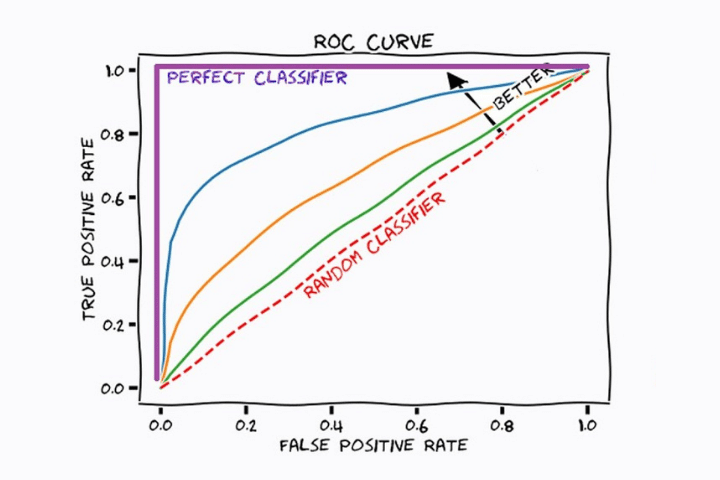
\includegraphics[width=0.8\textwidth]{curva-roc.png}
\end{figure}

La curva ROC es una herramienta muy útil para evaluar el rendimiento de clasificadores binarios. En el gráfico podemos observar que:

\begin{itemize}
    \item El eje X representa la Tasa de Falsos Positivos (FPR)
    \item El eje Y representa la Tasa de Verdaderos Positivos (TPR) o Recall
    \item La línea punteada diagonal representa el clasificador aleatorio (AUC = 0.5)
    \item Las curvas de colores representan diferentes clasificadores
\end{itemize}

Cuanto más cerca esté la curva del punto (0,1), mejor será el rendimiento del clasificador. Un clasificador perfecto tendría un AUC de 1.0, mientras que un clasificador aleatorio tendría un AUC de 0.5.

\subsection{¿Cómo entiendo la curva ROC?}

Lo importante es pensar que para cada punto de umbral, existe una tasa de falsos positivos y una tasa de verdaderos positivos.

\subsection{Para un umbral de 0}

Para un umbral de 0, todos los casos son positivos y ninguno es negativo. Tendríamos una matriz de confusión de la siguiente forma:

\begin{center}
    \begin{tikzpicture}
    \draw (0,0) rectangle (4,4);
    \draw (0,2) -- (4,2);
    \draw (2,0) -- (2,4);
    
    \node[above] at (2,4) {\textbf{R}};
    \node[left] at (0,2) {\textbf{P}};
    
    \fill[green!30] (0,2) rectangle (2,4);
    \fill[red!30] (2,0) rectangle (4,2);
    \fill[blue!30] (0,0) rectangle (2,2);
    \fill[yellow!30] (2,2) rectangle (4,4);
    
    \node at (1,3) {$\alpha$ (VP)};
    \node at (3,3) {$\beta$ (FP)};
    \node at (1,1) {0 (FN)};
    \node at (3,1) {0 (VN)};
    
    \end{tikzpicture}
\end{center}

Cuando queramos ahora calcular para umbral 0, fijemonos bien que nunca va a importar cuando vale $\alpha$ o $\beta$, porque siempre lo otro va a ser 0.

\subsubsection{Punto que voy a poner en el eje X: FPR}

Recordemos que la FPR es:

\[
\text{FPR} = \frac{FP}{FP + VN}
\]

\vspace{0.3em}

Remplazando con los valores que podemos tener con un umbral 0, donde todos los casos son positivos y ninguno es negativo, tenemos que:

\[
\text{FPR} = \frac{FP}{FP + VN} = \frac{FP}{FP + 0} = 1
\]

\subsubsection{Punto que voy a poner en el eje Y: TPR}

Recordemos que la TPR es:

\[
\text{TPR} = \frac{VP}{VP + FN}
\]

\vspace{0.3em}

Remplazando con los valores que podemos tener con un umbral 0, donde todos los casos son positivos y ninguno es negativo, tenemos que:

\[
\text{TPR} = \frac{VP}{VP + FN} = \frac{VP}{VP + 0} = 1
\]

\subsection{Para un umbral de 1}

Para un umbral de 1, todos los casos son negativos y ninguno es positivo. Tendríamos una matriz de confusión de la siguiente forma:

\begin{center}
    \begin{tikzpicture}
    \draw (0,0) rectangle (4,4);
    \draw (0,2) -- (4,2);
    \draw (2,0) -- (2,4);
    
    \node[above] at (2,4) {\textbf{R}};  
    \node[left] at (0,2) {\textbf{P}};
    
    \fill[green!30] (0,2) rectangle (2,4);
    \fill[red!30] (2,0) rectangle (4,2);
    \fill[blue!30] (0,0) rectangle (2,2);
    \fill[yellow!30] (2,2) rectangle (4,4);
    
    \node at (1,3) {0 (VP)};
    \node at (3,3) {0 (FP)};
    \node at (1,1) {$\alpha$ (FN)};
    \node at (3,1) {$\beta$ (VN)};
    
    \end{tikzpicture}

\end{center}

Cuando queramos ahora calcular para umbral 1, fijemonos de vuelta bien que nunca va a importar cuanto vale $\alpha$ o $\beta$, porque siempre lo otro va a ser 0.

\subsubsection{Punto que voy a poner en el eje X: FPR}

Recordemos que la FPR es:

\[
\text{FPR} = \frac{FP}{FP + VN}
\]

\vspace{0.3em}

Remplazando con los valores que podemos tener con un umbral 1, donde ninguno es positivo y todos son negativos, tenemos que:

\[
\text{FPR} = \frac{FP}{FP + VN} = \frac{FP}{FP + 0} = 1
\]

\subsubsection{Punto que voy a poner en el eje Y: TPR}


Recordemos que la TPR es:

\[
\text{TPR} = \frac{VP}{VP + FN}
\]

\vspace{0.3em}

Remplazando con los valores que podemos tener con un umbral 1, donde ninguno es positivo y todos son negativos, tenemos que:

\[
\text{TPR} = \frac{VP}{VP + FN} = \frac{0}{0 + FN} = 0
\]

\subsubsection{Para un umbral \( U \)}

Para un umbral \( U \), tengo que calcular la FPR y la TPR para cada valor de umbral. Para obtener la curva ROC completa, necesito calcular estos valores para todos los posibles umbrales. Una curva perfecta es aquella en la que existe al menos un umbral tal que la separación entre clases es perfecta, es decir, no hay falsos positivos ni falsos negativos.

\subsection{Curva PR}

La curva PR es prácticamente igual a la curva ROC, solo que en el eje X tenemos la precisión y en el eje Y tenemos el recall. Todo se calcula igual que con la curva ROC, solo que en vez de usar la FPR y la TPR, usamos la precisión y el recall. Tendremos que agarrar un umbral \( U \) y calcular la precisión y el recall para ese umbral, y así con todos.

\section{Casos de Uso y Recomendaciones}

\subsection{Salud}
En el ámbito de la salud, las consecuencias de un falso negativo (no detectar una enfermedad) son mucho más graves que las de un falso positivo. Por lo tanto:
\begin{itemize}
    \item Priorizar el recall sobre la precisión
    \item Usar curvas PR en lugar de ROC
    \item No usar accuracy como métrica principal
\end{itemize}

\subsection{Justicia}
En el sistema judicial, debemos considerar que es mejor dejar libre a un culpable que condenar a un inocente, entonces:
\begin{itemize}
    \item Usar curvas ROC para evaluar el balance
    \item Considerar el impacto social de los errores
    \item Evaluar la transparencia y explicabilidad del modelo
\end{itemize}

\section{Ejemplo Práctico}
Consideremos un modelo de detección de enfermedades cardíacas con los siguientes resultados:

\begin{center}
\begin{tikzpicture}
\draw (0,0) rectangle (4,4);
\draw (0,2) -- (4,2);
\draw (2,0) -- (2,4);

\node[above] at (2,4) {\textbf{R}};
\node[left] at (0,2) {\textbf{P}};

\fill[green!30] (0,2) rectangle (2,4);
\fill[red!30] (2,0) rectangle (4,2);
\fill[blue!30] (0,0) rectangle (2,2);
\fill[yellow!30] (2,2) rectangle (4,4);

\node at (1,3) {80};
\node at (3,3) {20};
\node at (1,1) {10};
\node at (3,1) {90};

\end{tikzpicture}
\end{center}

Calculemos todas las métricas:
\begin{align*}
\text{Accuracy} &= \frac{80 + 90}{200} = 0.85 \\
\text{Precision} &= \frac{80}{90} = 0.89 \\
\text{Specificity (TNR)} &= \frac{90}{100} = 0.90 \\
\text{Recall (TPR)} &= \frac{80}{100} = 0.80 \\
\text{Fall-out (FPR)} &= \frac{10}{100} = 0.10 \\
\text{Miss Rate (FNR)} &= \frac{20}{100} = 0.20 \\
\text{F1} &= 2 \times \frac{0.89 \times 0.80}{0.89 + 0.80} = 0.84 \\
\text{FDR} &= \frac{10}{90} = 0.11 \\
\text{FOR} &= \frac{20}{110} = 0.18 \\
\text{NPV} &= \frac{90}{110} = 0.82
\end{align*}

En este caso, aunque la accuracy es alta (0.85), el recall de 0.80 significa que estamos perdiendo el 20\% de los casos positivos, lo cual no está bueno en un problema médico. La tasa de falsos positivos (FPR) es del 10\%, lo que significa que estamos clasificando incorrectamente como enfermos al 10\% de las personas sanas.

\section{Implementación en Python}

\begin{lstlisting}[language=Python]
from sklearn.metrics import accuracy_score, precision_score
from sklearn.metrics import recall_score, f1_score
from sklearn.metrics import confusion_matrix
from sklearn.metrics import roc_curve, auc
from sklearn.metrics import precision_recall_curve

# Metricas basicas
accuracy = accuracy_score(y_true, y_pred)
precision = precision_score(y_true, y_pred)
recall = recall_score(y_true, y_pred)
f1 = f1_score(y_true, y_pred)

# Matriz de confusion
conf_matrix = confusion_matrix(y_true, y_pred)

# Curva ROC
fpr, tpr, _ = roc_curve(y_true, y_pred_proba)
roc_auc = auc(fpr, tpr)

# Curva PR
precision, recall, _ = precision_recall_curve(
    y_true, y_pred_proba
)
\end{lstlisting}

\end{document}
